\begin{figure*}[h!]
	
	\begin{center}
		\begin{tabular}{ c  c  c  c   }
			%\hline
			\hspace*{-1.5cm} \multirow{4}{*}[-0in]{ \rotatebox[origin=t]{0}{ {\vspace{10in} \includegraphics[height=.35\linewidth]{figures/uvcoverage/uv_eht2017.pdf}}
					\qquad  }} &  \hspace{-1cm} \large{\textsf{True Static Image}}   &\large{\textsf{MEM \& TV Recon.}} &\large{\textsf{CHIRP Recon.}}      \\
			&\hspace{-1cm} {{\includegraphics[height=.16\linewidth]{figures/singleimage/hotakaframe.pdf}} } &
			{\includegraphics[height=.16\linewidth]{figures/singleimage/hotakaframe_andrew.pdf}} &
			{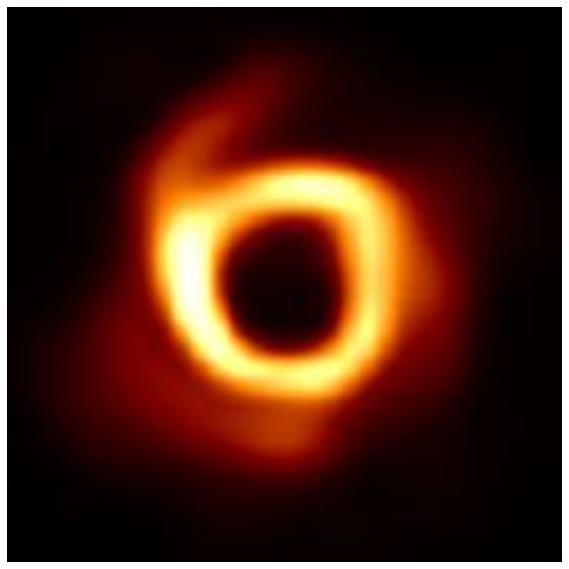
\includegraphics[height=.16\linewidth]{figures/singleimage/hotakaframe_chirp.pdf}} 
			\\
			& \vspace{-.1in}
			\\
			& \hspace{-1cm} \large{\textsf{Gauss Recon.}}   &\large{\textsf{Clipped Gauss Recon.}} &\large{\textsf{Estimated SNR} }     \\
			&\hspace{-1cm} {{\includegraphics[height=.16\linewidth]{figures/singleimage/hotakaframe_gauss.pdf}} } &
			\includegraphics[height=.16\linewidth]{figures/singleimage/hotakaframe_gaussnneg.pdf} &
			\includegraphics[height=.16\linewidth]{figures/singleimage/hotakaframe_gausssnr.pdf} 
			\\
		\end{tabular}
		\caption{{\bf Static Imaging Comparison:} Results of static imaging using a multivariate Gaussian prior (a=2) compared to state-of-the-art reconstruction methods using MEM \& TV regularizers~\cite{andrew} as well as patch-based regularizers (CHIRP)~\cite{bouman2016computational}. Data is generated using a static image with the uv-coverage of the EHT2017 array shown on the left (see Section~\ref{sec:results}). The uv-coverage is colored by time, as indicated by the colorbar in Figure~\ref{fig:uvcov2} \michael{I'm not sure the journal will let you forward reference a figure.}. In addition to realistic thermal noise, atmospheric phase errors have been included in the data. Although the previous algorithms (MEM \& TV and CHIRP) both produce better results, the Gaussian reconstruction is able to correctly get the broad structure of the underlying image. Since we do not impose positivity, negative values are reconstructed. However, by clipping the resulting image we can see that the result aligns well with the true static image. The Gaussian prior model also allows us to easily estimate the SNR of our reconstruction using the diagonal entries of the posterior covariance matrix. \michael{I don't understand how to interpret the SNR. Also, why is it in dB? Is it a relative value among image pixels? The SNR seems to be lowest in regions of the images that are reliably reconstructed...)}} 
		\label{fig:staticimaging}
	\end{center}
\end{figure*}
